\documentclass[11pt,aspectratio=43,usenames,dvipsnames]{beamer}
\usepackage[utf8]{inputenc}
\usepackage{amsmath, amsfonts, amssymb, amsthm}
\usepackage[T1]{fontenc}
% mint: code chuck and syntax highlighting
%% outputdir should change according to pdf build directory
\usepackage[outputdir=build,cache=false]{minted}
\usepackage{lmodern}
\usepackage{xcolor}
\usepackage{setspace}
\usepackage{booktabs}
\usepackage{multirow}
\usepackage{graphicx}
\usepackage{fontawesome}

\usepackage[mode=tex]{standalone}
\usepackage{tikz}
\usetikzlibrary{decorations}
\usetikzlibrary{decorations.pathreplacing, intersections}
\usepackage{pgfplots}
\usetikzlibrary{calc,positioning}
\usepgfplotslibrary{fillbetween}
\pgfplotsset{compat=newest, scale only axis, width = 10cm}

% ---------------------------------------------------------------------
% Coordinate extraction
% #1: node name
% #2: output macro name: x coordinate
% #3: output macro name: y coordinate
\newcommand{\Getxycoords}[3]{%
    \pgfplotsextra{%
        % using `\pgfplotspointgetcoordinates' stores the (axis)
        % coordinates in `data point' which then can be called by
        % `\pgfkeysvalueof' or `\pgfkeysgetvalue'
        \pgfplotspointgetcoordinates{(#1)}%
        % `\global' (a TeX macro and not a TikZ/PGFPlots one) allows to
        % store the values globally
         \global\pgfkeysgetvalue{/data point/x}{#2}%
         \global\pgfkeysgetvalue{/data point/y}{#3}%
     }%
}
% ---------------------------------------------------------------------

\usepackage{ulem}
\usepackage{hyperref}
\usepackage{booktabs}
\usepackage{babel}
\usepackage{makecell}
\usepackage[para,online,flushleft]{threeparttable}
\usepackage{pdfpages}
\usepackage{tcolorbox}
\usepackage{bm}
\usepackage{appendixnumberbeamer}
\usepackage{natbib}
\usepackage{caption}
\captionsetup[figure]{labelformat=empty}% redefines the caption setup of the figures environment in the beamer class.
\usetheme[compress]{Boadilla}
\usecolortheme{default}
\useoutertheme{miniframes}
\usefonttheme[onlymath]{serif}

\newcommand{\jump}[2]{\hyperlink{#1}{\beamerbutton{#2}}}
\newcommand{\extjump}[2]{\href{#1}{\beamerbutton{#2}}}
\newcommand{\orange}[1]{\textcolor{orange}{#1}}
\newcommand{\red}[1]{\textcolor{red}{#1}}
\newcommand{\blue}[1]{\textcolor{blue}{#1}}
\newcommand{\green}[1]{\textcolor{OliveGreen}{#1}}

\renewcommand{\square}{\scalebox{0.7}{$\blacksquare$ \hspace{0.5em}}}
\setbeamertemplate{itemize item}{\raisebox{0.1em}{\scalebox{0.7}{$\blacksquare$}}}
\setbeamertemplate{itemize subitem}[circle]
\setbeamertemplate{itemize subsubitem}{--}
\setbeamercolor{itemize item}{fg=black}
\setbeamercolor{itemize subitem}{fg=black}
\setbeamercolor{itemize subsubitem}{fg=black}
\setbeamercolor{item projected}{bg=darkgray,fg=white}
\definecolor{blue}{rgb}{0.2, 0.2, 0.7}
\setbeamercolor{alerted text}{fg=blue}
\setbeamertemplate{enumerate items}[circle]


\setbeamertemplate{headline}{}

%==========================================
\let\olditemize=\itemize
\let\endolditemize=\enditemize
\renewenvironment{itemize}{\olditemize \itemsep1em}{\endolditemize}
\let\oldenumerate=\enumerate
\let\endoldenumerate=\endenumerate
\renewenvironment{enumerate}{\oldenumerate \itemsep1em}{ \endoldenumerate}

\DeclareMathOperator*{\argmax}{\arg\!\max}
\DeclareMathOperator*{\E}{\mathbb{E}}
\DeclareMathOperator*{\var}{\rm Var}
\DeclareMathOperator*{\cov}{\rm Cov}

\theoremstyle{definition}
\newtheorem{assume}{Assumption}
\newtheorem{lem}{Lemma}
\newtheorem{proposition}{Proposition}
\newtheorem{thm}{Theorem}
\newtheorem{corol}{Corollary}

\AtBeginSection[]{
  \begin{frame}[noframenumbering]
  \vfill
  \centering
  \begin{beamercolorbox}[sep=8pt,center,shadow=true,rounded=true]{title}
    \usebeamerfont{title}\insertsection\par%
  \end{beamercolorbox}
  \vfill
  \end{frame}
}

\begin{document}
    \title[Unit 16]{Unit 16 \\ Technological Progress, Unemployment, and Living Standards in the Long Run}
    \author[Hui-Jun Chen]{Hui-Jun Chen}
    \institute[OSU]{The Ohio State University}
    % \date{\today}
    \date{\today}
    \setbeamertemplate{navigation symbols}{}
    \setstretch{1.2}

%-------------------------------------------------------
{
%	\usebackgroundtemplate{\includegraphics[width=1\paperwidth]{../EveningSky_cropped_edit43_bright.jpg}}
    \begin{frame}
% \vspace{3em}
        \centering
%		{\footnotesize 	ECON 4002 Intermediate Macroeconomic Theory}
        \maketitle
% \vspace{-1.5em}
% \centering
% \includegraphics[width=0.55\linewidth]{Pictures/houses.jpeg}


    \end{frame}
}

% -------------------------------------------
\setbeamertemplate{headline}
{
\setbeamercolor{section in head/foot}{fg=black, bg=white}
\vskip1em \tiny \insertsectionnavigationhorizontal{1\paperwidth}{\hspace{0.50\paperwidth}}{}
}
%------------------------------------------

\section[Intro]{Introduction}
\label{sec:Introduction}

\begin{frame}{Introduction \extjump{https://www.core-econ.org/the-economy/book/text/16.html}{Textbook}}
\label{slide:Introduction}

\begin{columns}
    \begin{column}{0.3\textwidth}
        \begin{itemize}
            \item<only@1> Tech change long-run living standards $ \uparrow  $ yet cause short-run unemployment
            \item<only@1> Cross-countries of unemployment cannot be explained by innovation
            \item<only@2> Production has become more capital intensive, without resulting in mass unemployment. How could this outcome occur?
        \end{itemize}
    \end{column}
    \begin{column}{0.7\textwidth}
        \begin{figure}
            \centering
            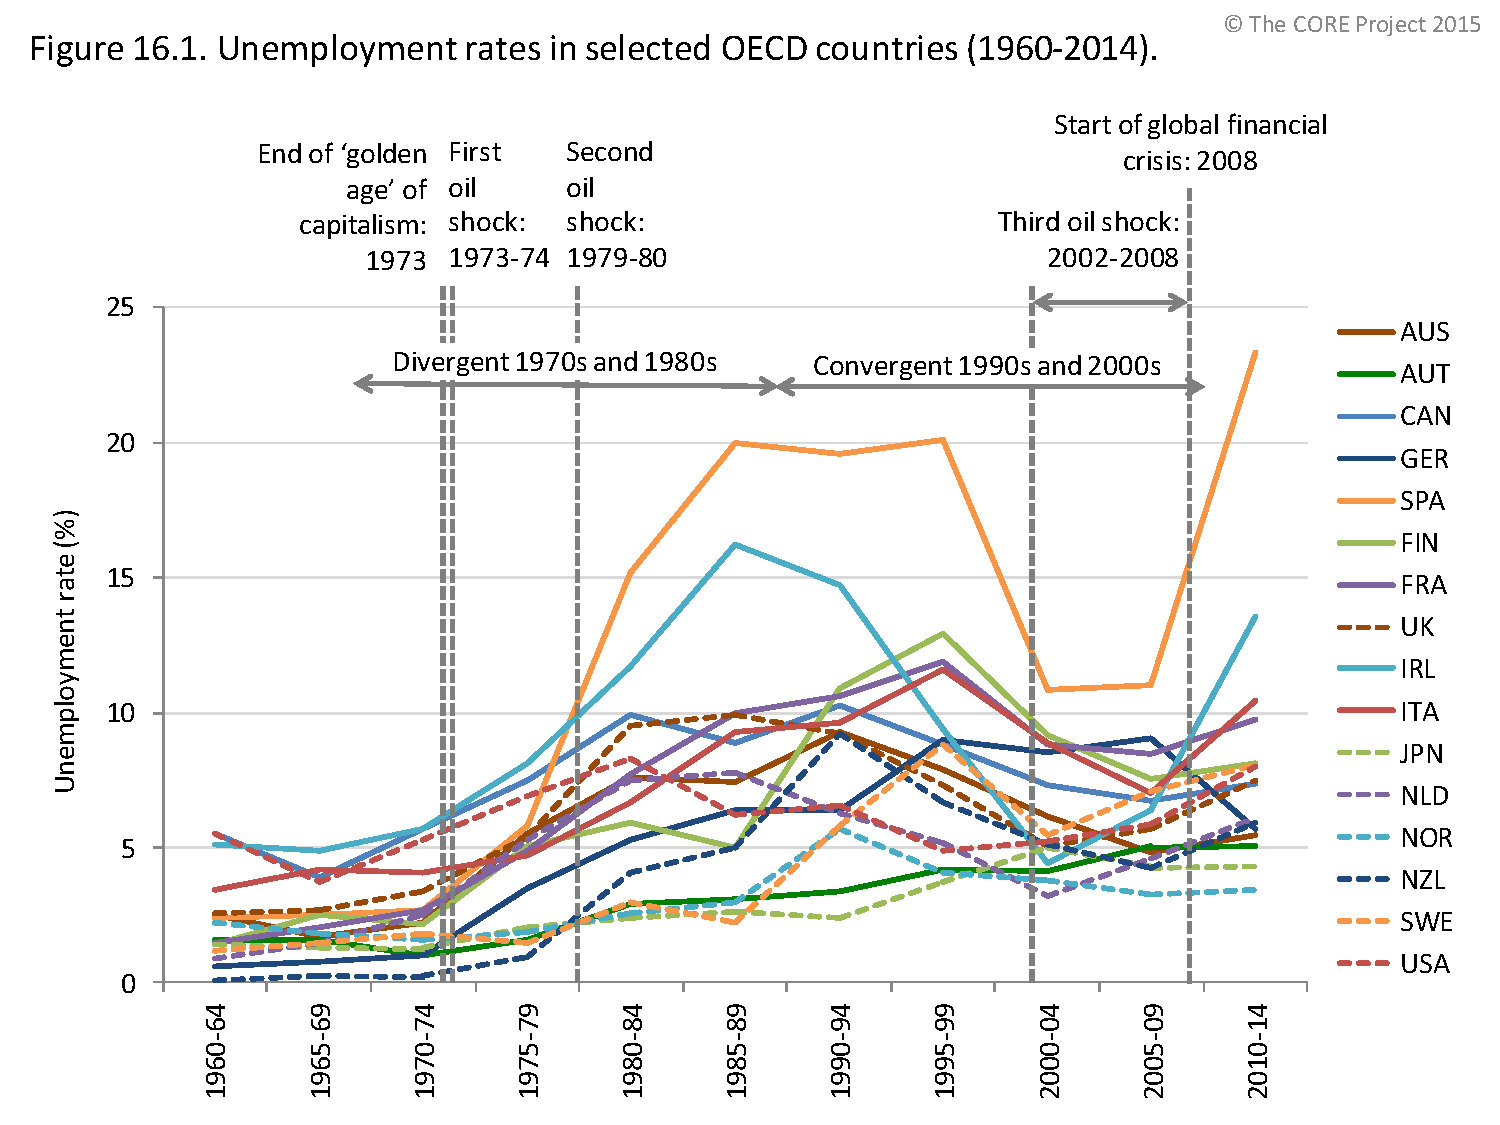
\includegraphics[width=\textwidth]{./figures/2.pdf}
        \end{figure}

    \end{column}
\end{columns}

    \begin{center}
        How can institutions and policies explain these differences?
    \end{center}

\end{frame}

\begin{frame}{Structure of Units}
\label{slide:Structure_of_Units}
    \begin{figure}
        \centering
        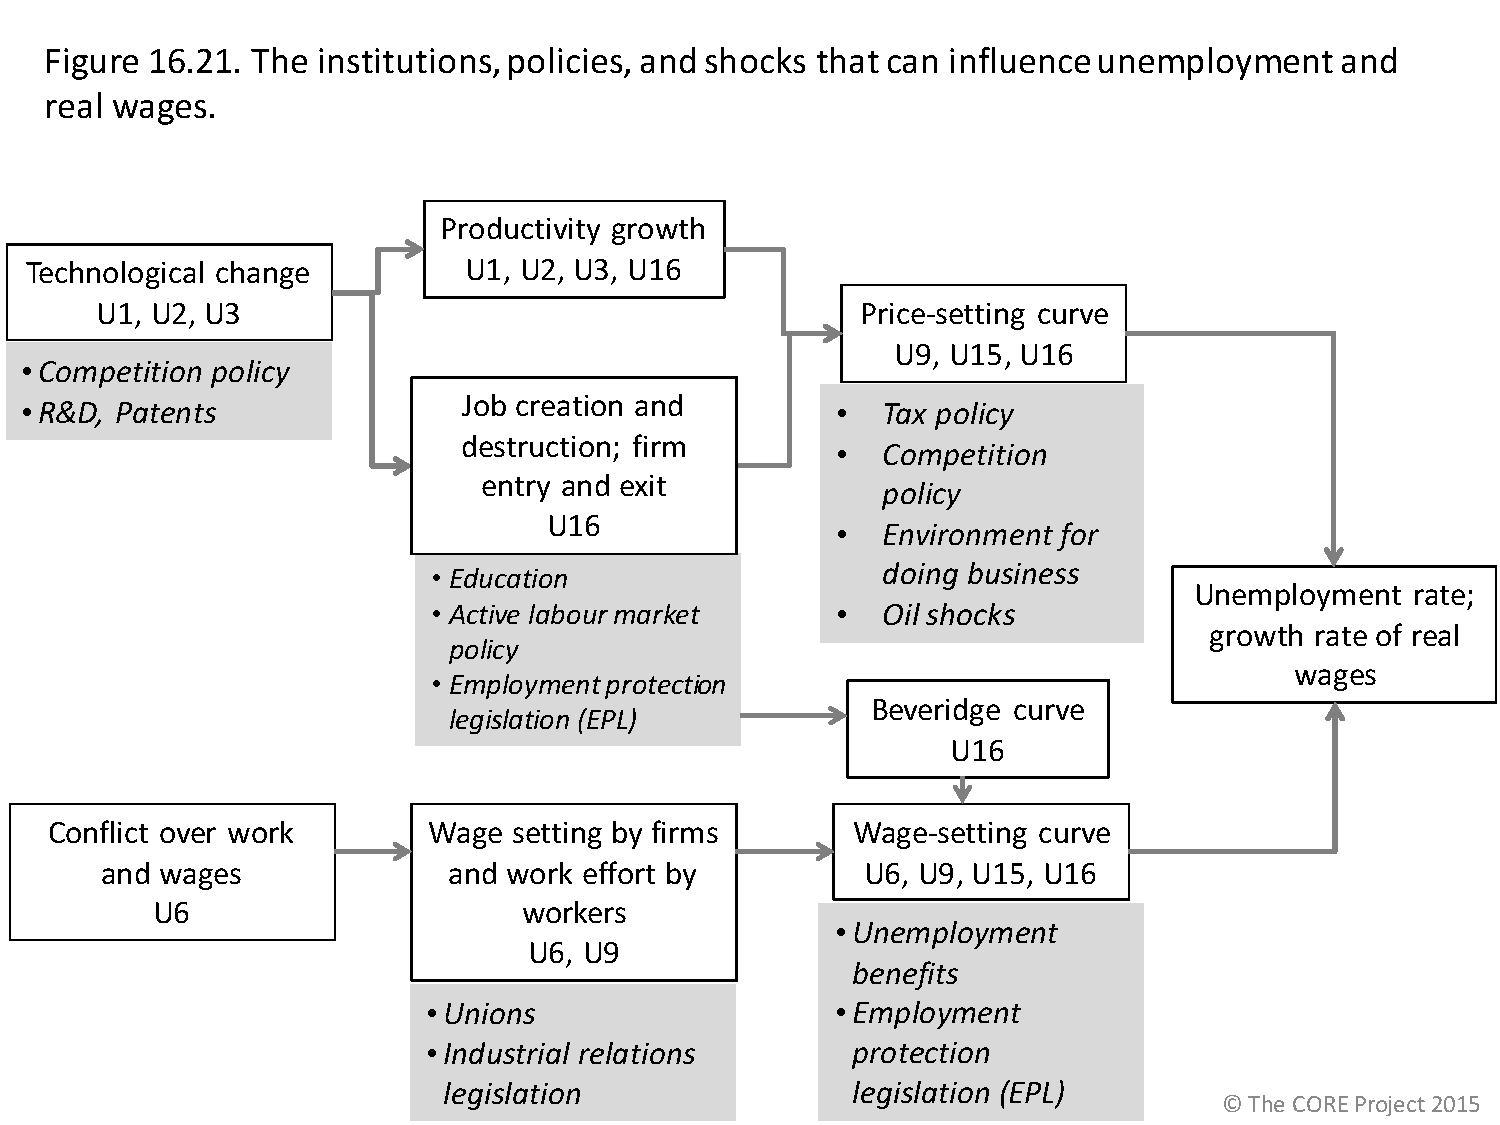
\includegraphics[width=.85\textwidth]{./figures/20.pdf}
    \end{figure}

\end{frame}

\section[\faIndustry]{Job Creation and Unemployment}
\label{sec:Job_Creation_and_Unemployment}

\begin{frame}{Technological progress and living standards}
\label{slide:Technological_progress_and_living_standards}
    \begin{itemize}
        \item Firms can earn \textbf{innovation rents} by introducing new technology.
        \item Firms that cannot keep up with innovation eventually fail
        \begin{itemize}
            \item $ \Rightarrow  $ Schumpeter: creative destruction
        \end{itemize}
        \item New technologies require new machines
        \item Technological advance relies on capital-intensive methods of production to be profitable.
        \item This process allows a sustained increase in average living standards.
    \end{itemize}

\end{frame}

\begin{frame}{Classical Growth Model: Decreasing MPK}
\label{slide:Classical_Growth_Model__Decreasing_MPK}
    \begin{figure}
        \centering
        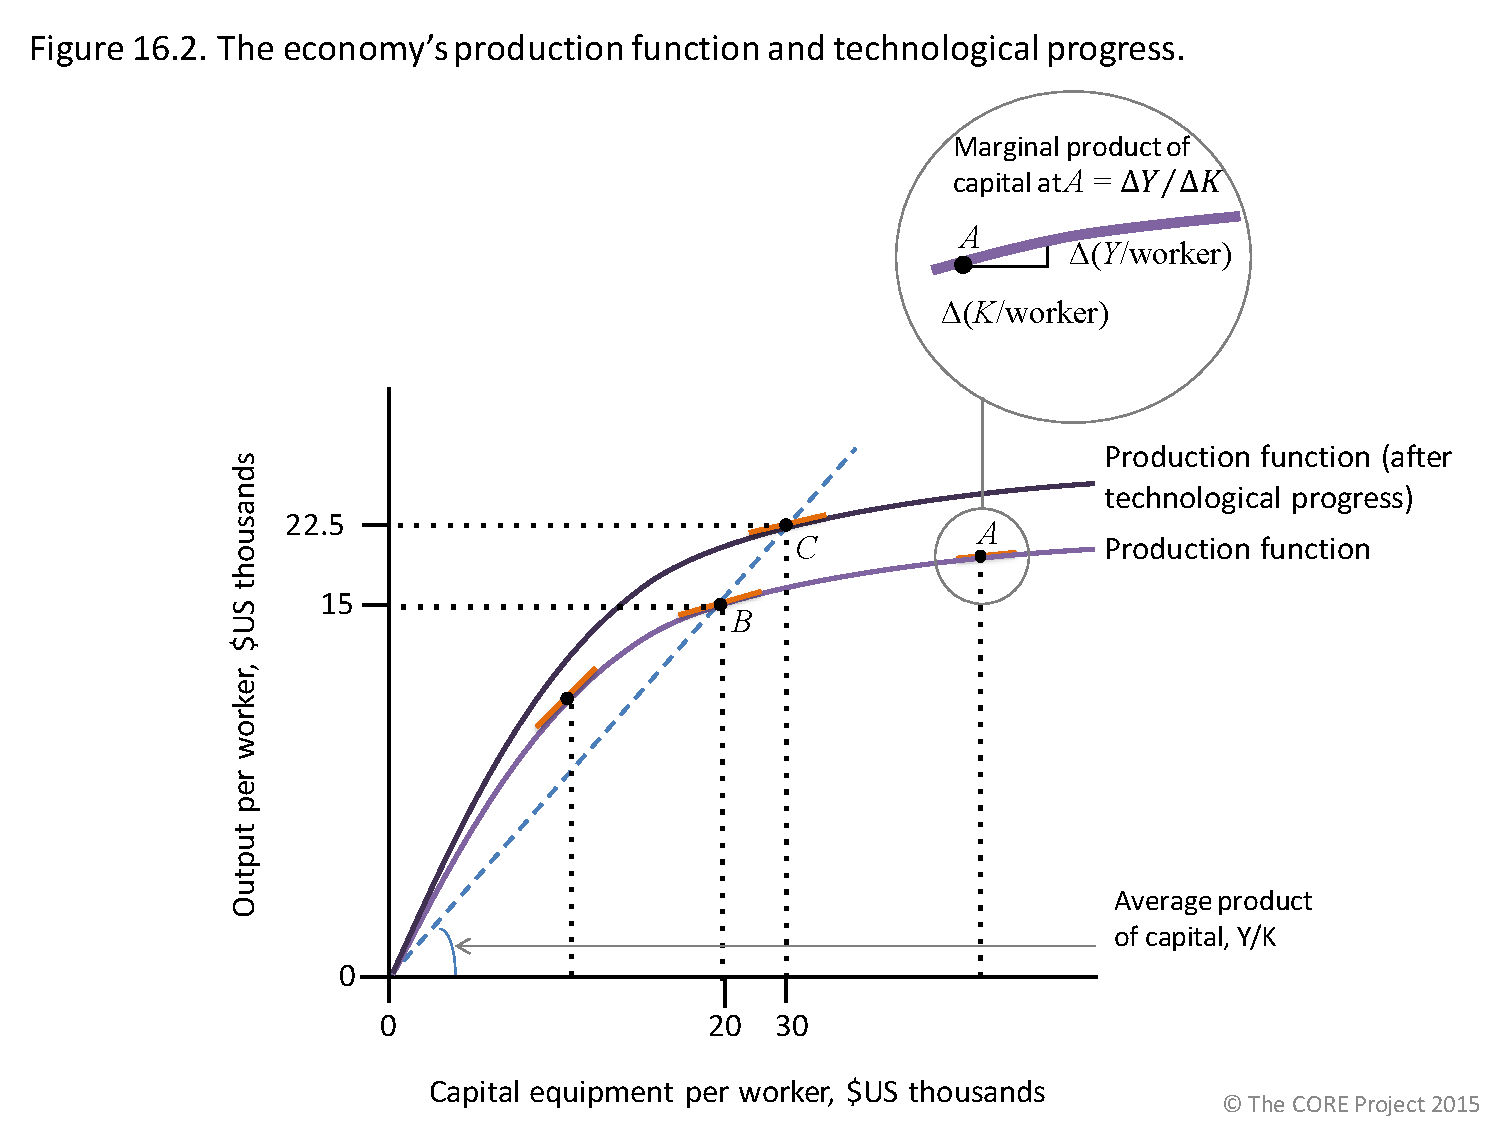
\includegraphics[width=.9\textwidth]{./figures/3.pdf}
    \end{figure}

\end{frame}

\begin{frame}{Technological progress over time}
\label{slide:Technological_progress_over_time}
    \begin{figure}
        \centering
        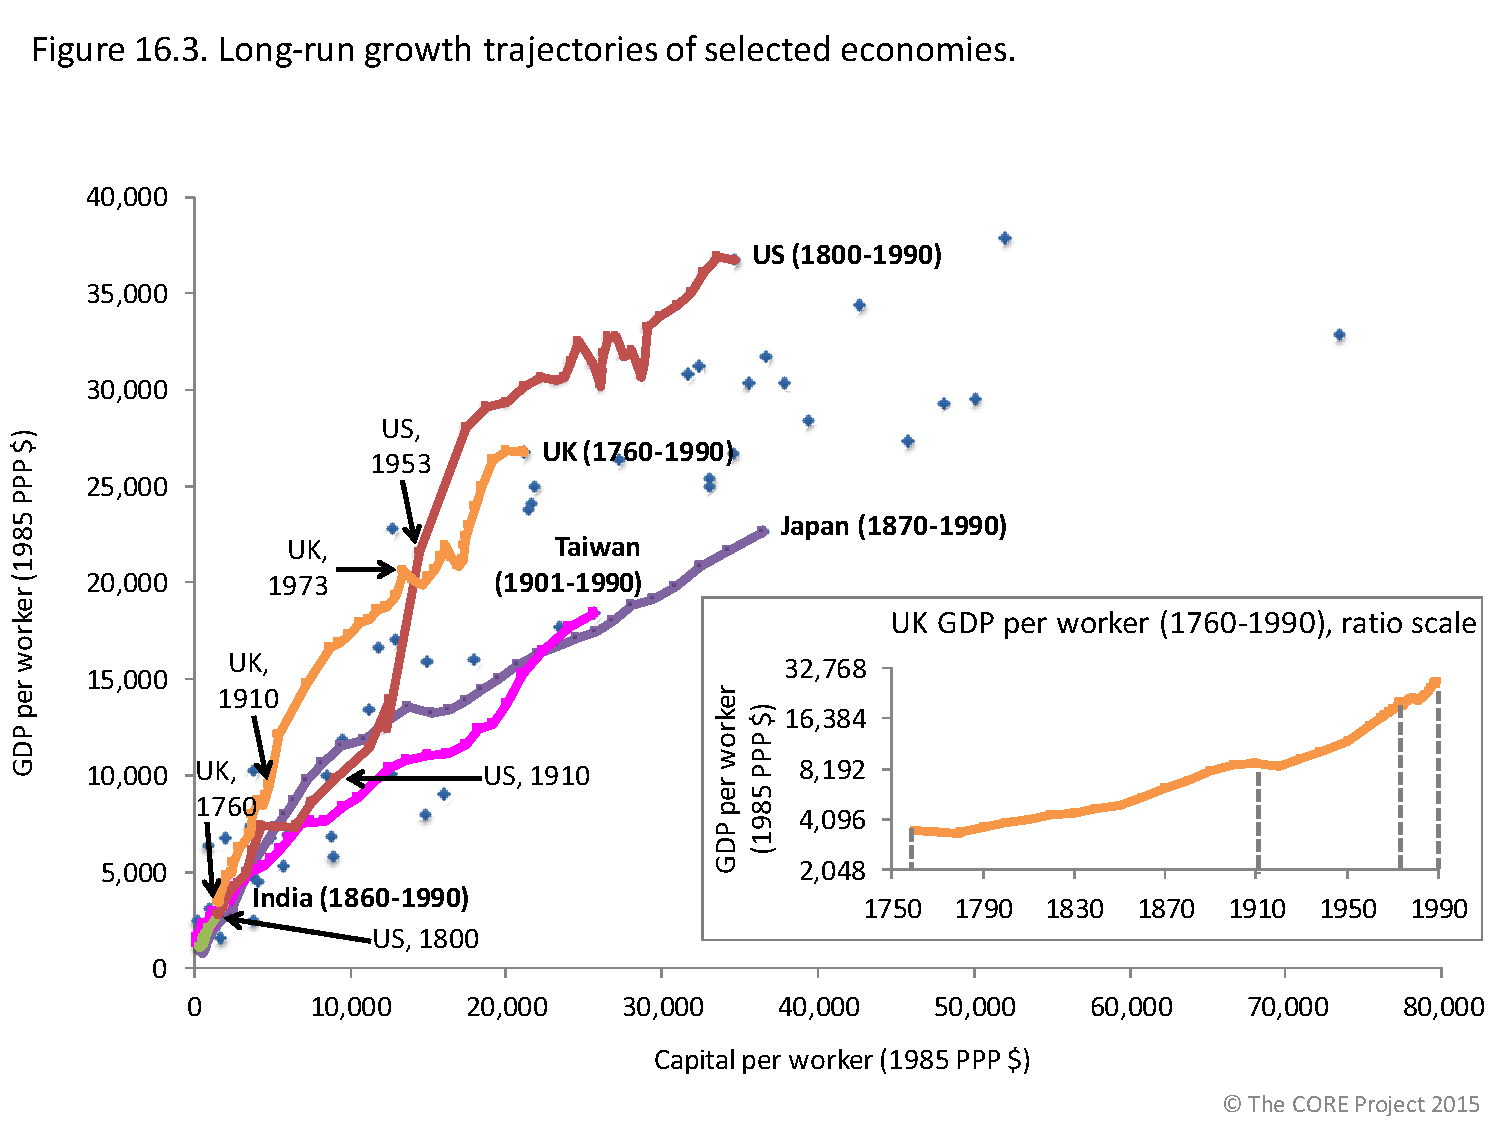
\includegraphics[width=.8\textwidth]{./figures/4.pdf}
        \caption{capital productivity remained roughly constant, why?}
    \end{figure}

\end{frame}

\begin{frame}{Job creation/destruction}
\label{slide:Job_creation_destruction}
    \begin{figure}
        \centering
        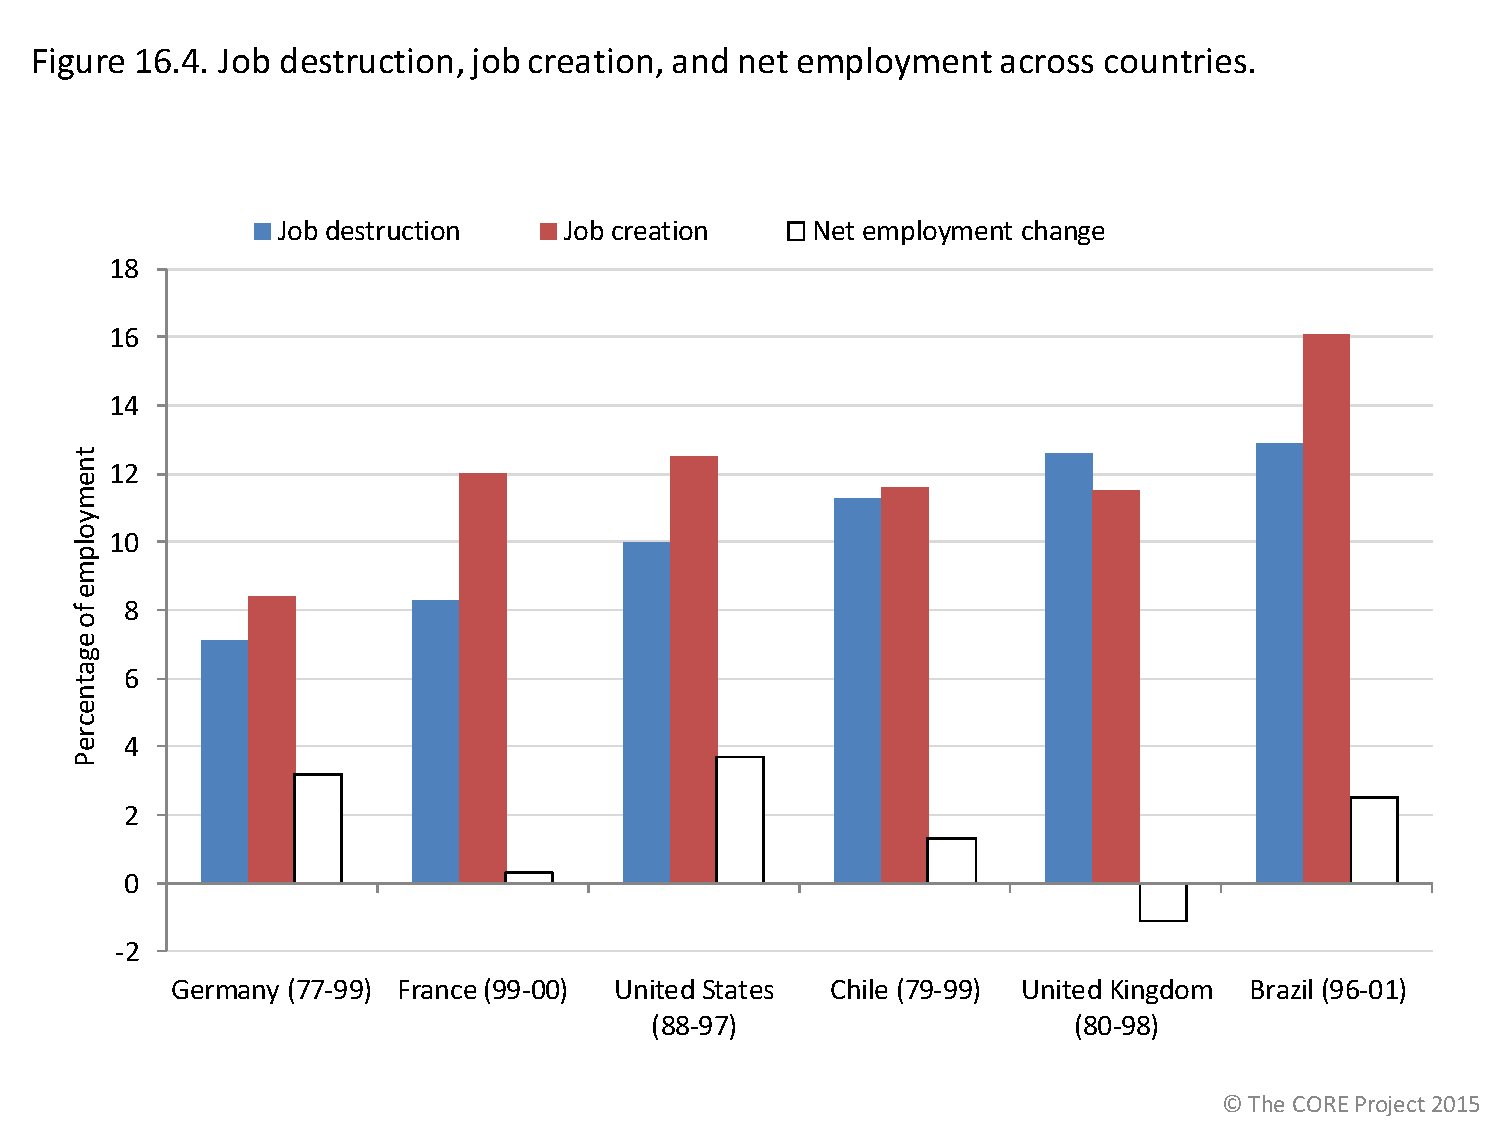
\includegraphics[width=.6\textwidth]{./figures/6.pdf}
    \end{figure}
    \begin{itemize}
        \item Labour-saving technological progress can also create jobs
        \item e.g. reallocation of work from low- to high-productivity firms
        \item Net employment change = job creation – job destruction
    \end{itemize}
\end{frame}

\begin{frame}{The Beveridge Curve}
\label{slide:The_Beveridge_Curve}
\begin{columns}
    \begin{column}{0.4\textwidth}
        \begin{itemize}
            \item<only@1> \textbf{Def}: inverse relationship between the \alert{unemployment rate} and the \alert{job vacancy rate}
            \item<only@1> Recession:  post fewer vacancies and lay off more workers
            \item<only@1> Boom:  post more vacancies and need more workers
            \item<only@2> German Beveridge curve shifted closer to the origin due to reforms that helped unemployed workers find jobs.
            \item<only@2>  US curve shifted away from the origin due to a skill-based mismatch and limited worker mobility.
        \end{itemize}


    \end{column}
    \begin{column}{0.6\textwidth}
        \begin{figure}
            \centering
            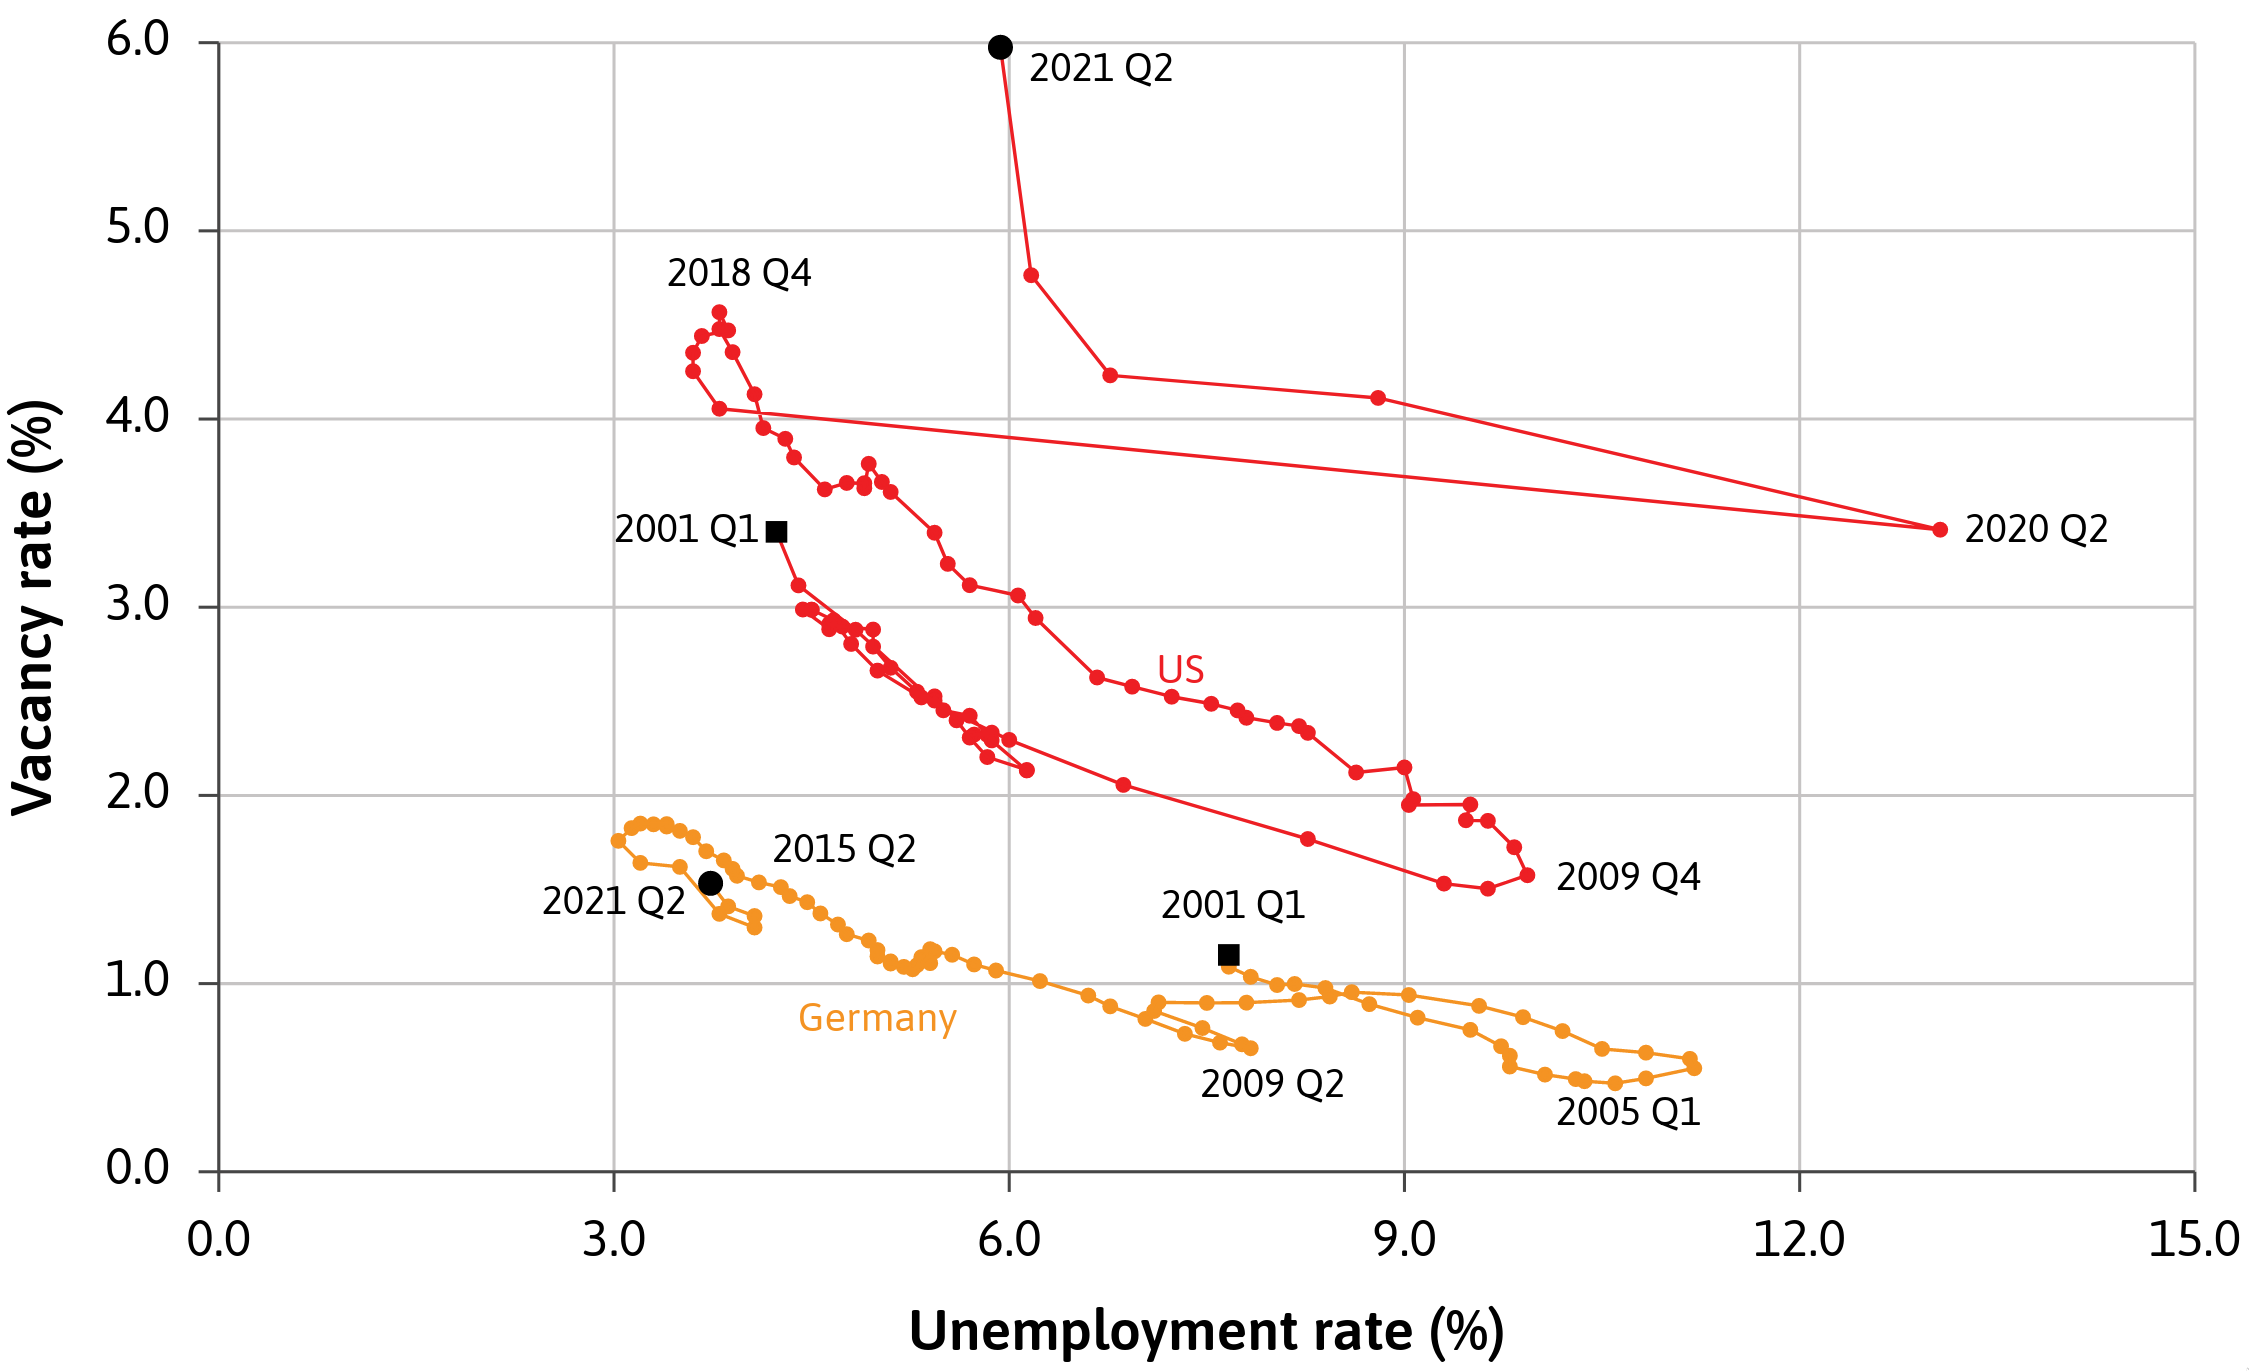
\includegraphics[width=\textwidth]{./figures/pic-selected-230326-2202-54.png}
        \end{figure}

    \end{column}
\end{columns}

\end{frame}

\begin{frame}{Labor Market Matching}
\label{slide:Labor_Market_Matching}
    \begin{center}
        Beveridge curve can shift over time!
    \end{center}
    \begin{itemize}
        \item $ \because $ changes in the labour market matching efficiency
        \item \alert{Skill Mismatch}: the unemployed may not have the \alert{skills required} for the job jobseekers
        \item \alert{Geographical constraint}: vacancies may be located in different parts of the country
        \item Policies and technology can improve efficiency
    \end{itemize}

\end{frame}

\section[\faWrench]{Long-run Labor Market Model}
\label{sec:Long_run_Labor_Market_Model}

\begin{frame}{Long-run unemployment}
\label{slide:Long_run_unemployment}
\begin{itemize}
    \item In the long run, firms can enter/exit (so capital stock can change)
    \item \alert{Work incentives}: depend on \textbf{wage-setting curve}
    \item \alert{Investment incentives}: depend on \textbf{price-setting curve}
    \item \alert{Long-run equilibrium} in the labour market is when
    \begin{enumerate}
        \item wages,
        \item employment level, and
        \item the number of firms are constant
    \end{enumerate}


\end{itemize}

\end{frame}

\begin{frame}{Equilibrium Profit}
\label{slide:Equilibrium_Profit}
    \begin{columns}
        \begin{column}{0.3\textwidth}
            \begin{itemize}
                \item<only@1> Profit determines the number of firms in the market.
                \item<only@1> High markup = firms enter
                \item<only@1> lower markup = firms exit.
                \item<only@2> Self-correcting process:
                \item<only@2> more firms
                \item<only@2> = more competition
                \item<only@2> = higher elasticity of demand
                \item<only@2> = lower markup
                \item<only@2> = fewer firms
            \end{itemize}
        \end{column}
        \begin{column}{0.7\textwidth}
            \begin{figure}
                \centering
                \only<1>{
                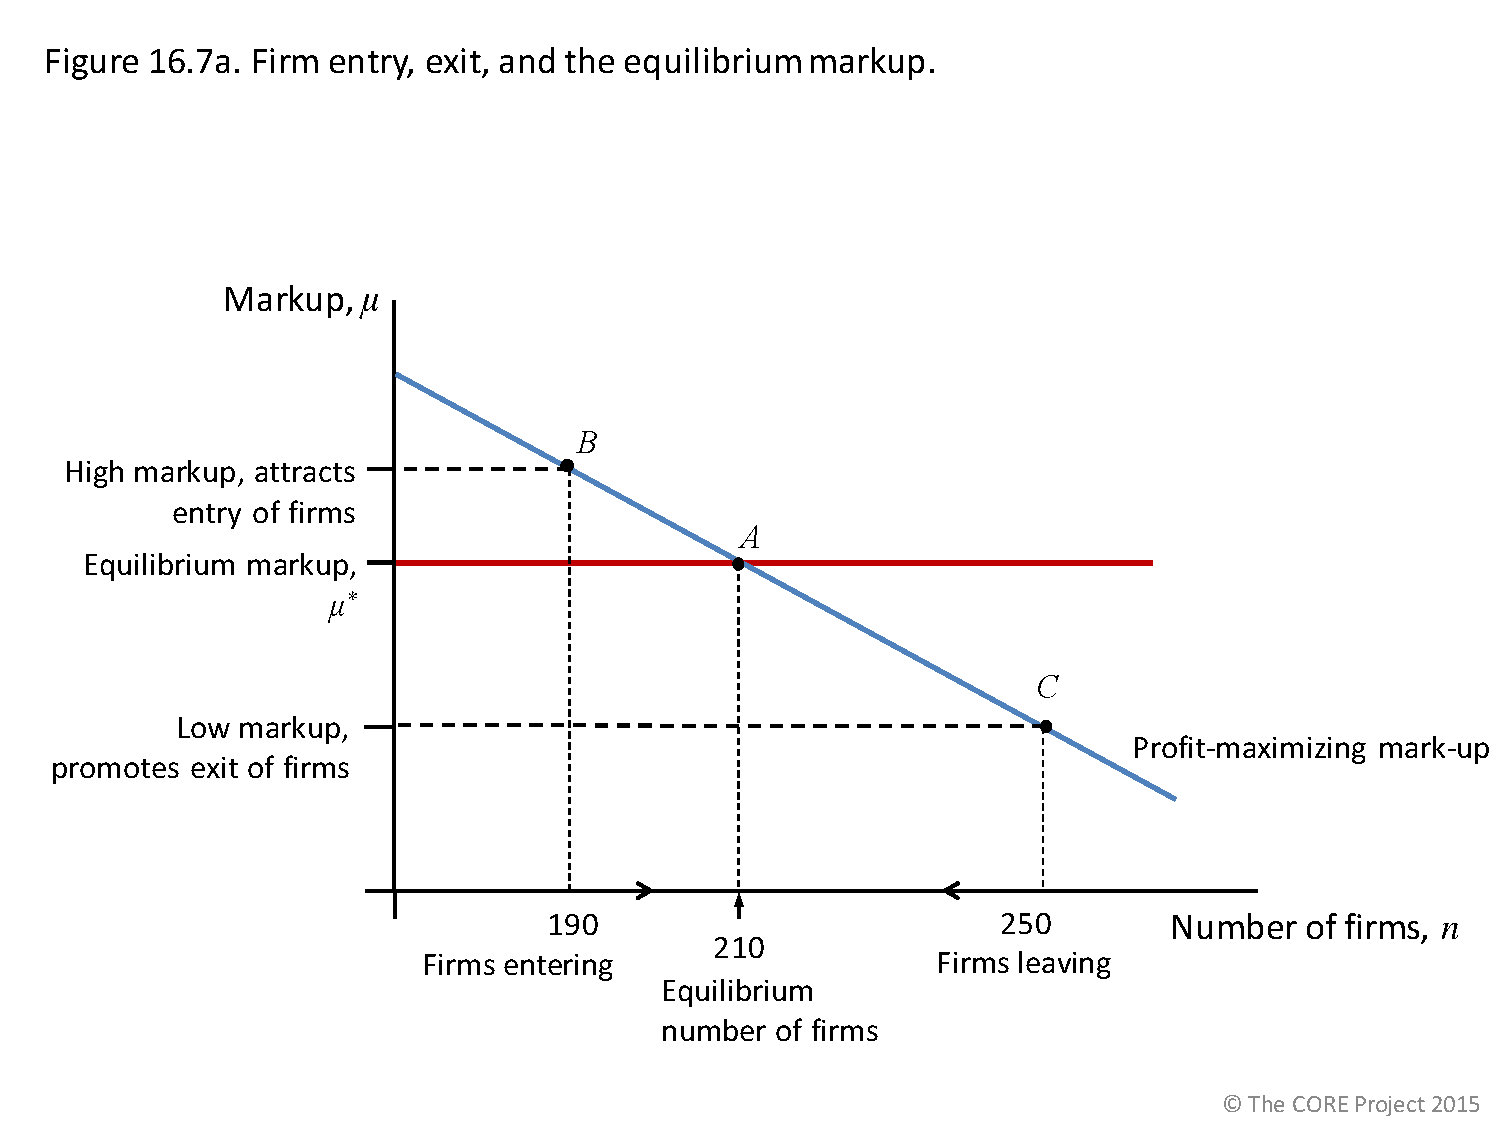
\includegraphics[width=\textwidth]{./figures/7.pdf}
                }
                \only<2>{
                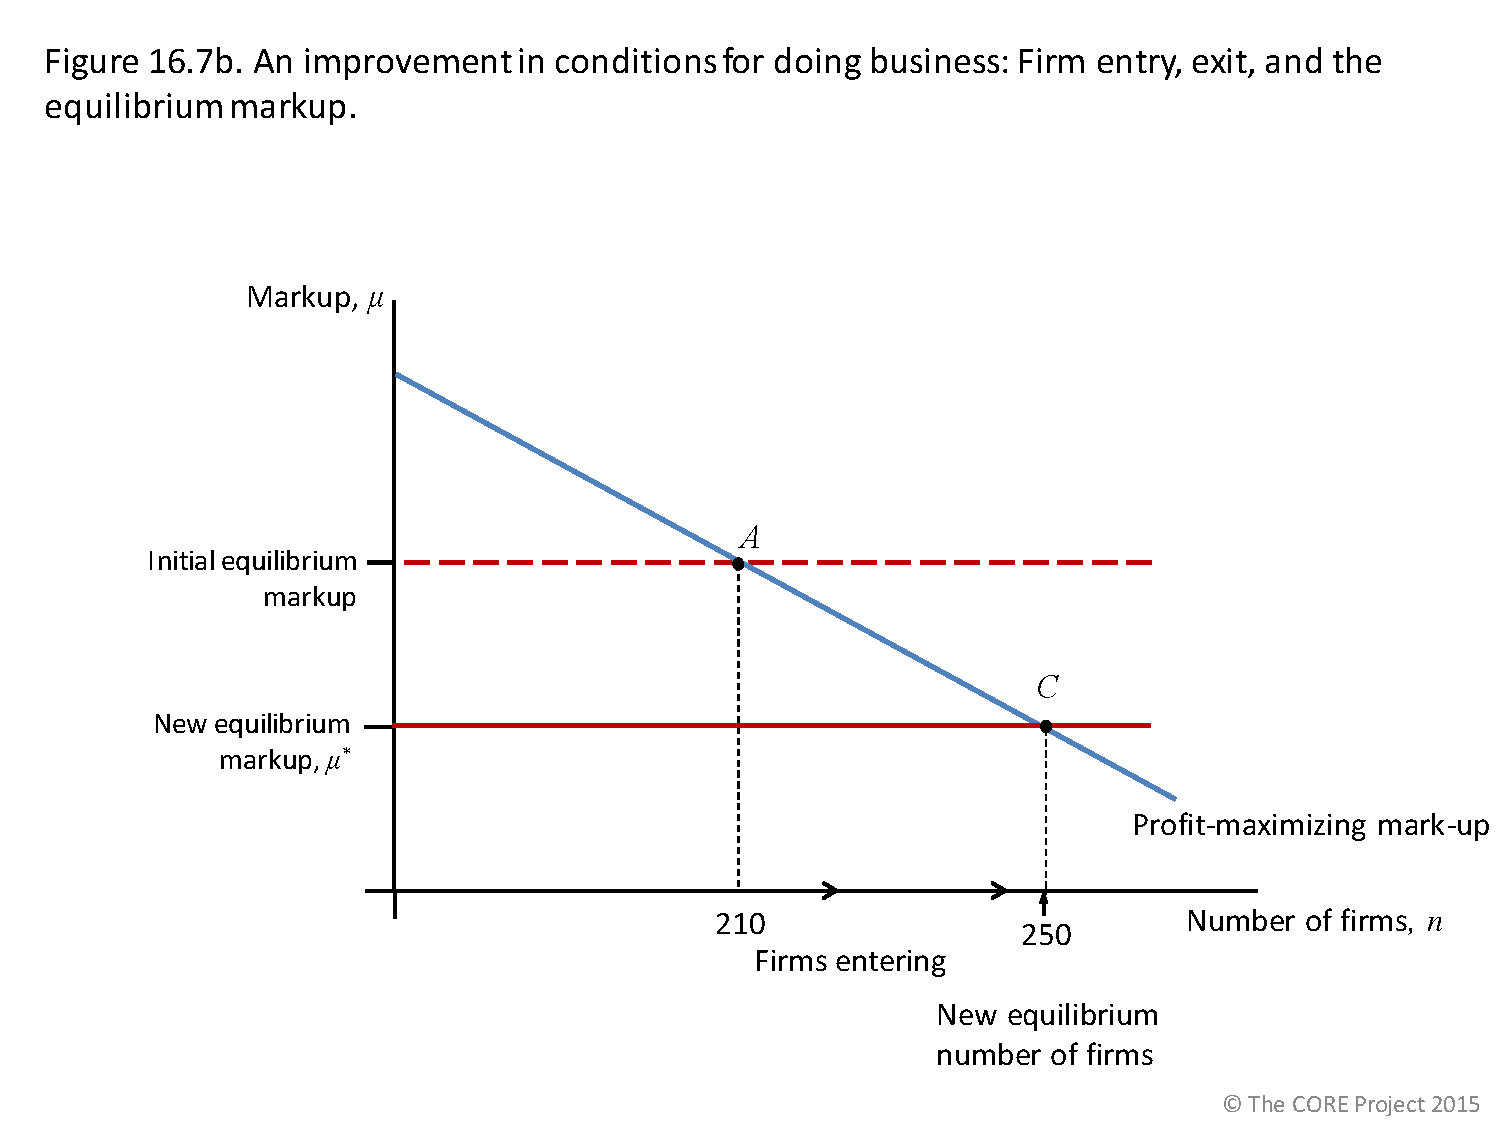
\includegraphics[width=\textwidth]{./figures/8.pdf}
                \begin{center}
                    Equilibrium profits can change: \\ e.g. property protection legislation
                \end{center}
                }
            \end{figure}
        \end{column}
    \end{columns}

\end{frame}

\begin{frame}{Long-run price-setting curve}
\label{slide:Long_run_price_setting_curve}
    \begin{columns}
        \begin{column}{0.3\textwidth}
            \begin{itemize}
                \small
                \item<only@1> Real wage depends on productivity ($\lambda$) and equilibrium profits ($\mu^{*}$).
                \item<only@1> Long-run price-setting curve: $w = \lambda(1 - \mu^{*})$
                \item<only@1> The price-setting curve depends on:
                \item<only@2> Expected long-run tax rates
                \item<only@2> Competition
                \item<only@2> Risk of expropriation
                \item<only@2> Quality of human capital/infrastructure
                \item<only@2> Opportunity cost of capital
                \item<only@2> Expected material costs
            \end{itemize}
        \end{column}
        \begin{column}{0.7\textwidth}
            \begin{figure}
                \centering
                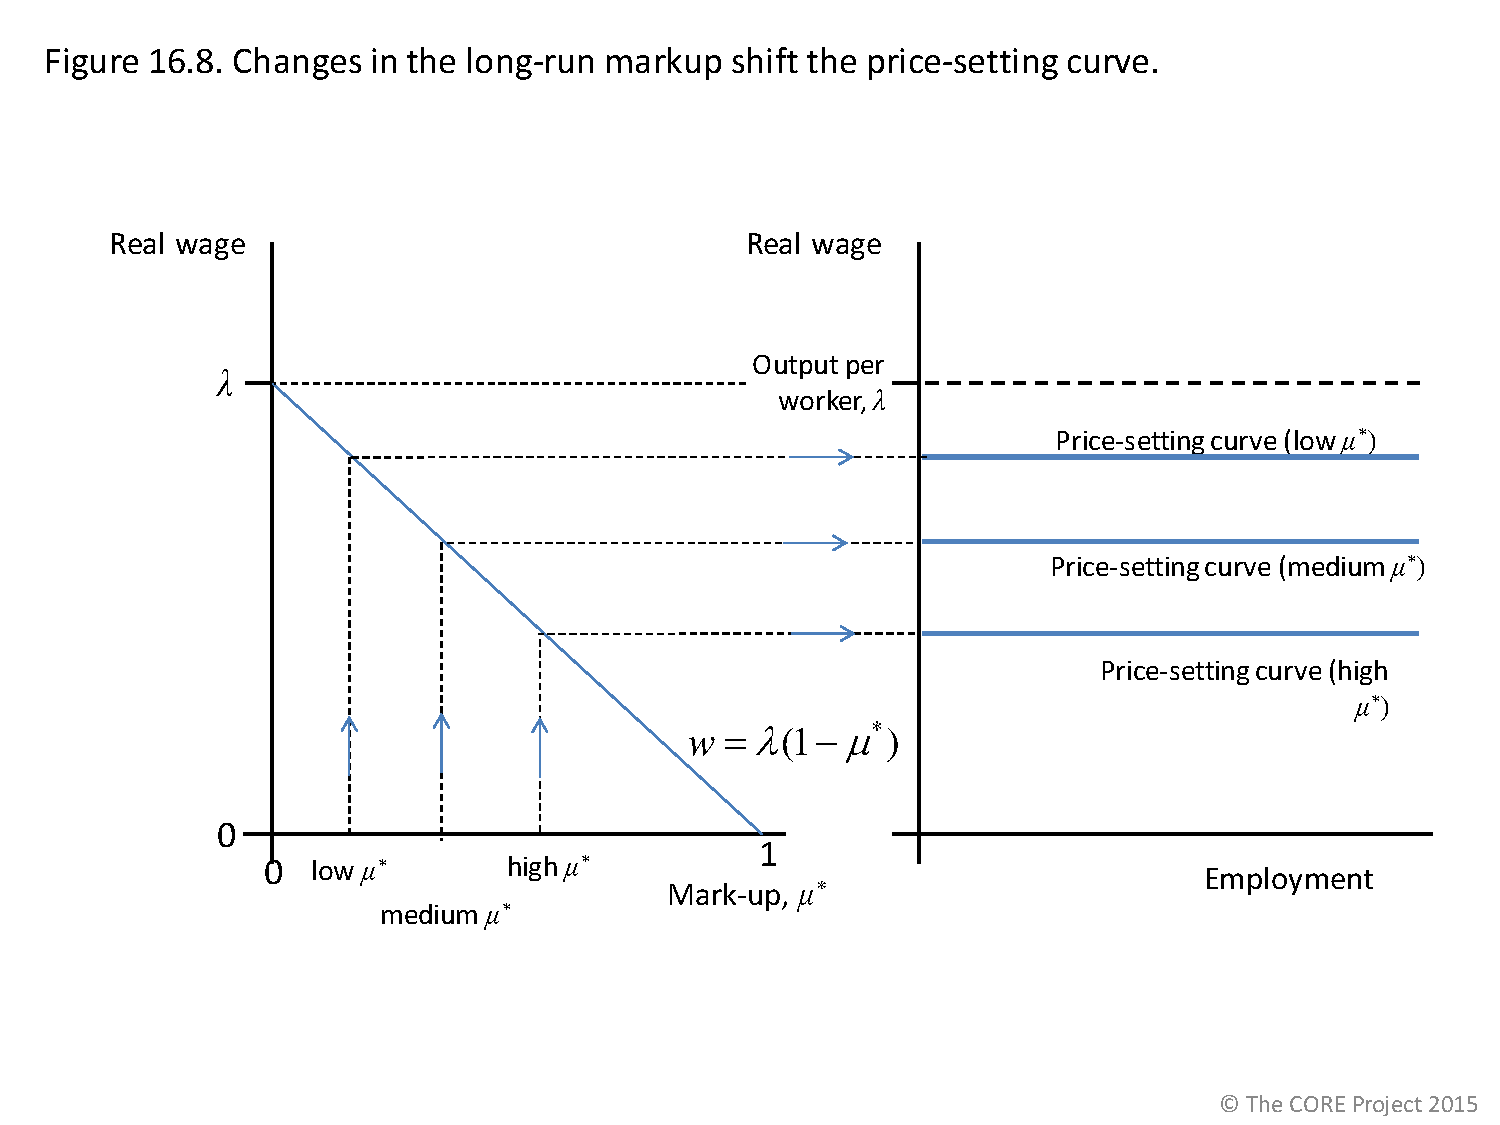
\includegraphics[width=\textwidth]{./figures/9.pdf}
            \end{figure}

        \end{column}
    \end{columns}

\end{frame}

\begin{frame}{Technological Improvement}
\label{slide:Technological_Improvement}
    \begin{columns}
        \begin{column}{0.3\textwidth}
            \begin{itemize}
                \item<only@1> New technology can increase both real wages and employment in the long-run.
                \item<only@1> The adjustment process takes time, and may involve job destruction in the short-run.
                \item<only@2> \textbf{Adjustment gap}: The lag between outside change in labor mkt conditions and the movement to the new equilibrium.
                \item<only@2> \textbf{Diffusion gap}: time for whole economy to adopt the innovation
            \end{itemize}
        \end{column}
        \begin{column}{0.7\textwidth}
            \begin{figure}
                \centering
                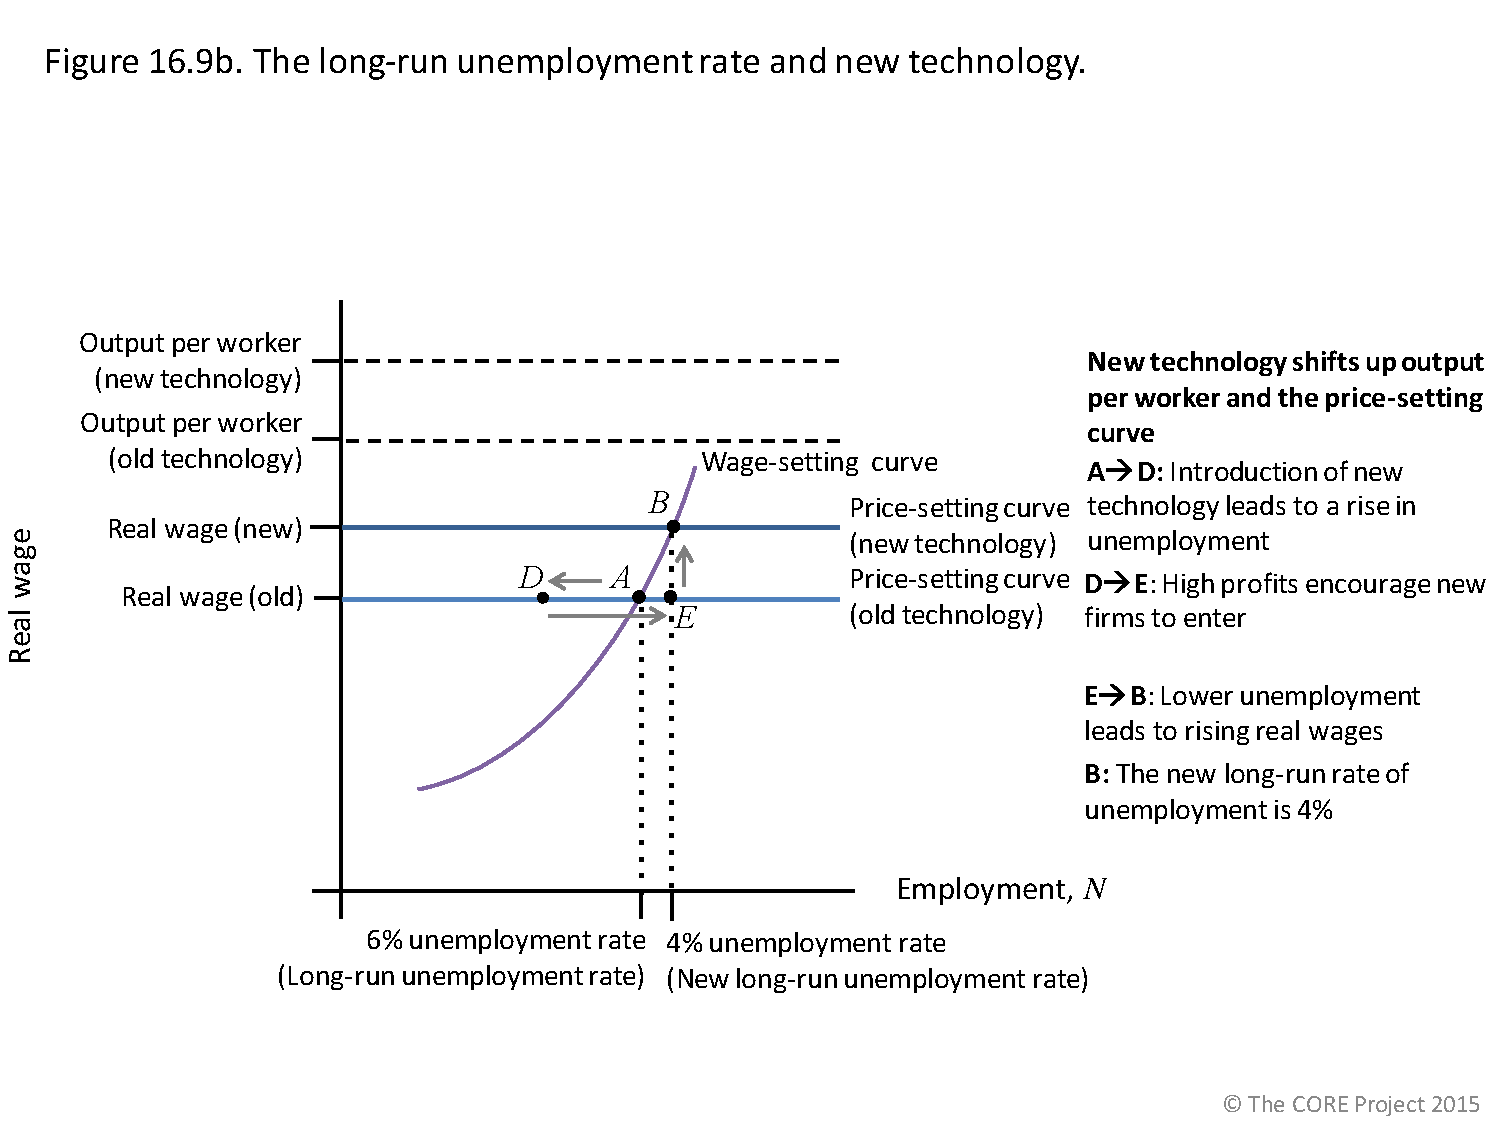
\includegraphics[width=\textwidth]{./figures/11.pdf}
            \end{figure}

        \end{column}
    \end{columns}

\end{frame}

\begin{frame}{Long-run wage-setting curve}
\label{slide:Long_run_wage_setting_curve}
\begin{center}
Unemployment does not continuously fall with technological progress because the \textbf{wage-setting curve can shift upwards}.
\end{center}

Technological change can indirectly shift the wage-setting curve due to:
\begin{itemize}
    \item Fair shares bargaining by unions
    \item Policies to help those affected e.g. employment protection laws
    \item Greater disutility of effort
    \item Improvement in the reservation wage
\end{itemize}

\end{frame}

\begin{frame}{Long Run v.s. Short Run}
\label{slide:Long_Run_v_s__Short_Run}
    \begin{figure}
        \centering
        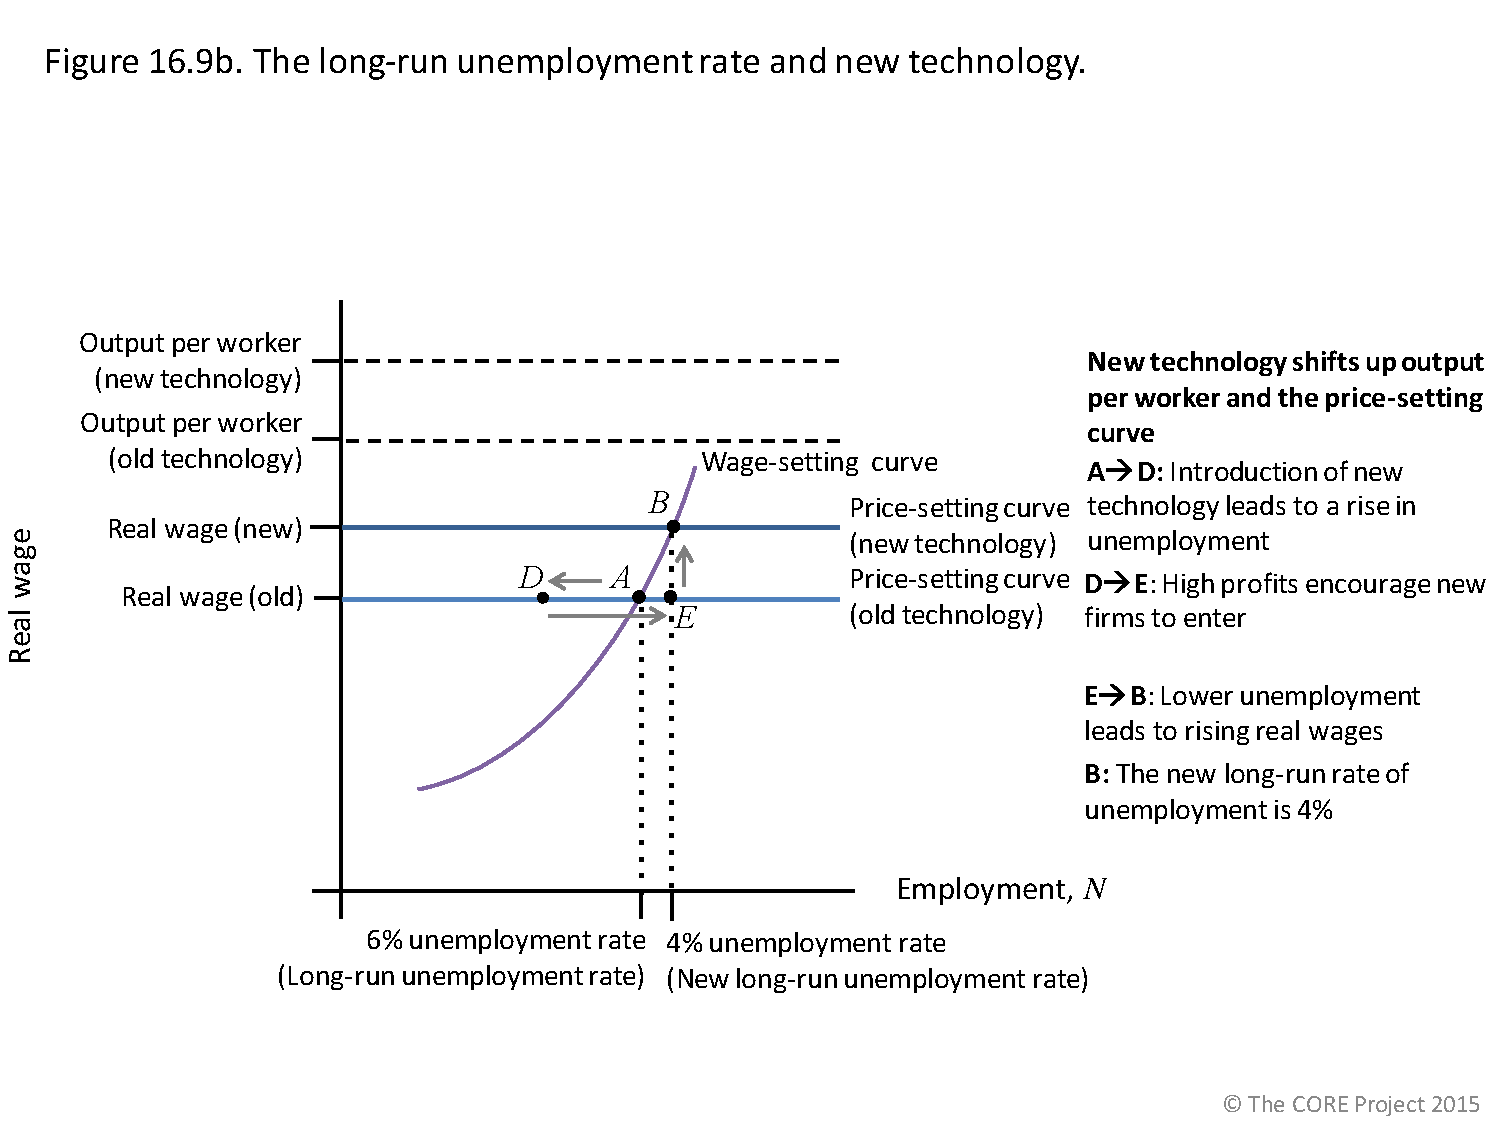
\includegraphics[trim={0cm 2cm 0cm 5cm}, clip, width=\textwidth]{./figures/11.pdf}
    \end{figure}

    \footnotesize
    \begin{tabular}{rlllll}
        \toprule
            & In Fig
            & Employment
            & Unemployment
            & Wage share
            & Inequality
        \\
        \hline
        \hline
        Short run
            & A $ \rightarrow  $ D
            & Down
            & Up
            & Down
            & Up
        \\
        \hline
        Long run
            & A $ \rightarrow  $ B
            & Up
            & Down
            & No change
            & Slightly Down
        \\
        \bottomrule
    \end{tabular}
    \normalsize

\end{frame}

\begin{frame}{Effect on Inequality}
\label{slide:Effect_on_Inequality}
    \begin{columns}
        \begin{column}{0.4\textwidth}
             Technological change increased inequality in the short run but reduced inequality in the long run:
             \begin{itemize}
                 \item Employees’ share of output returned to initial levels due to an increase in real wages
                 \item The higher real wage motivated employees to work hard at a lower
level of unemployment.
             \end{itemize}
        \end{column}
        \begin{column}{0.6\textwidth}
            \begin{figure}
                \centering
                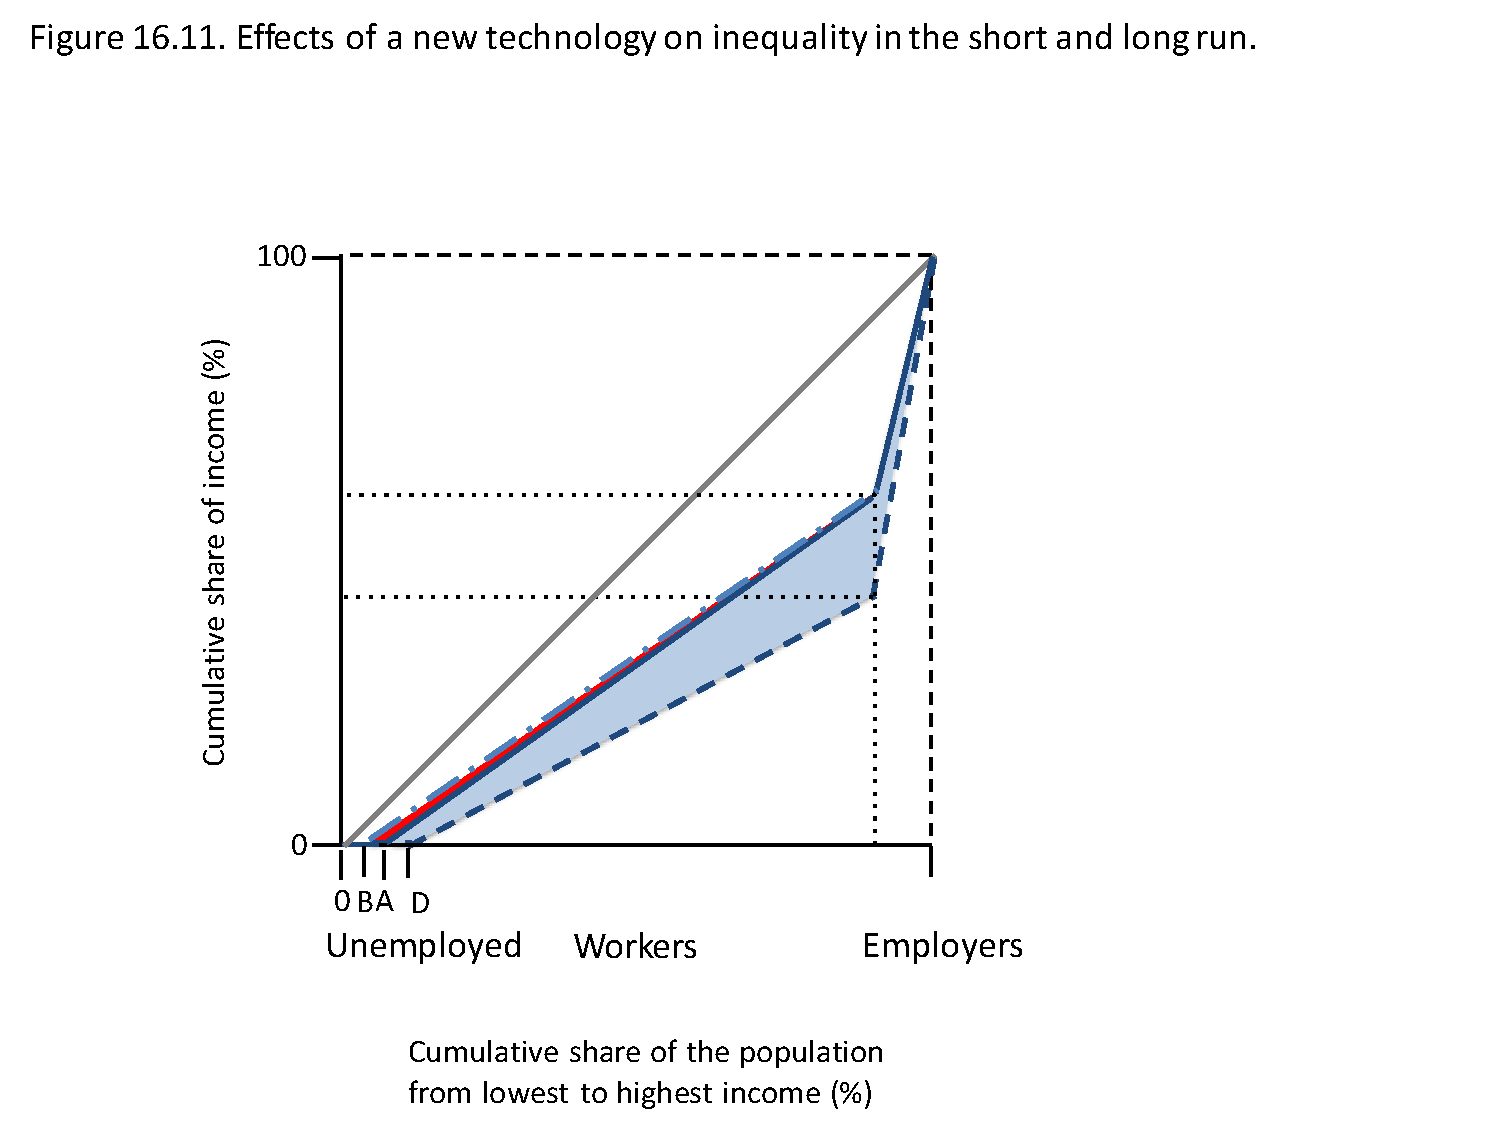
\includegraphics[width=\textwidth]{./figures/13.pdf}
            \end{figure}

        \end{column}
    \end{columns}

\end{frame}

\begin{frame}{How long is the long run?}
\label{slide:How_long_is_the_long_run_}
    The economy can go through a long adjustment process before reaching the new long-run equilibrium.
    \begin{example}
        Adjustment of the US labor markets to the Chinese import shock.
    \end{example}
    \begin{itemize}
        \item Many economists thought that this shock would not have a major negative effect on wages or employment, because workers in import-competing sectors could easily relocate to other regions.
        \item However, they underestimated the size of the shock and overestimated the degree of labour mobility – 2.4 million jobs were lost, and the labour market is still adjusting.
    \end{itemize}

\end{frame}

\section[Policy]{The role of institutions and policies}
\label{sec:_The_role_of_institutions_and_policies}

\begin{frame}{Differences across countries}
\label{slide:Differences_across_countries}
    \begin{figure}
        \centering
        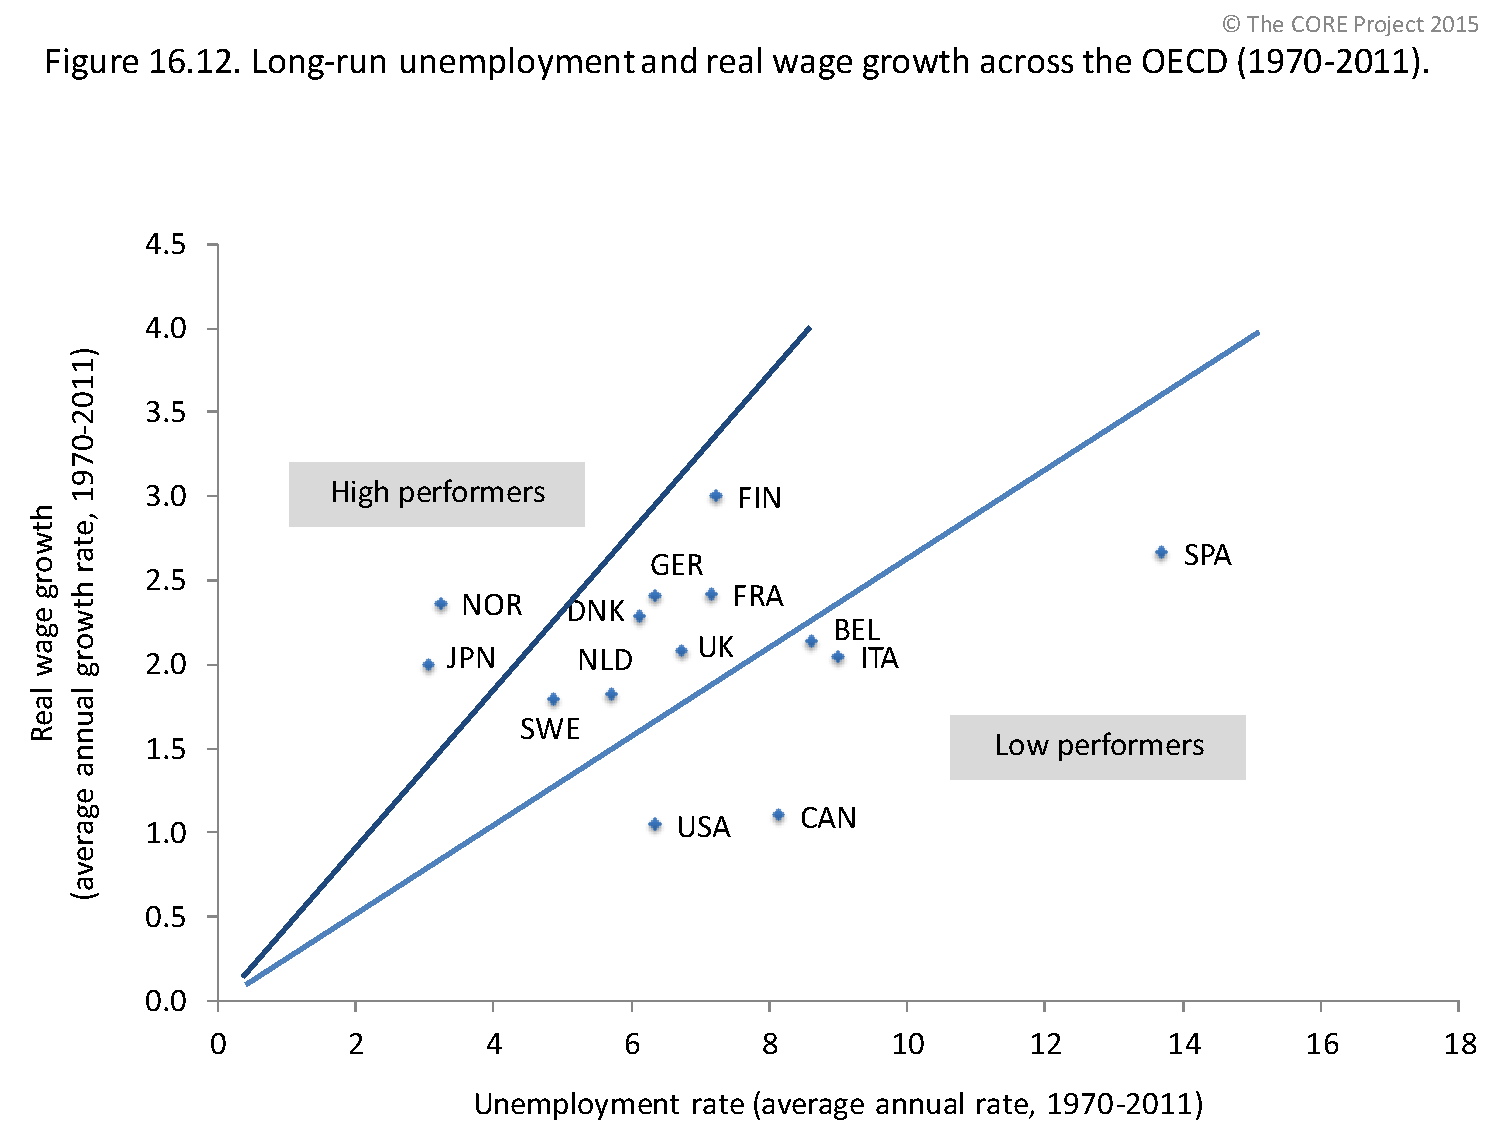
\includegraphics[width=.9\textwidth]{./figures/14.pdf}
    \end{figure}

\end{frame}

\begin{frame}{Important Factors}
\label{slide:Important_Factors}
    To achieve ``good'' economic performance, an economy must:
    \begin{enumerate}
        \item<1-4> Ensure price-setting curve shifts up more than wage-setting curve
        \item<2-4> Adjust rapidly and fully $ \Rightarrow  $ whole economy benefits from tech progress
    \end{enumerate}

    Possible explanation for cross-country differences are:
    \begin{enumerate}
        \item<3-4>  \alert{Institutions}: inclusive trade unions (represent many firms and sectors) choose not to exercise maximum bargaining power because wage increases affect job creation in the long run.
        \item<4-4> \alert{Policies}: well-designed unemployment insurance schemes and job placement services can achieve low unemployment rates.
    \end{enumerate}

        No magic formula: Institutions and policies used differ across successful countries and over time
\end{frame}

\begin{frame}{Examples}
\label{slide:Examples}
    \begin{enumerate}
        \item<1-3> Norway: Inclusive trade unions and employers’ associations set wage
demands in accordance with the productivity of labour, and also
supported legislation and policies that shifted the wage-setting curve
downwards, further expanding long-run unemployment.
        \item<2-3>
Japan: Employers’ associations coordinate wage setting across firms.
Corporations deliberately do not compete in hiring workers, to avoid
raising wages.
\item<3-3>
Spain: A combination of non-inclusive unions and government
legislation that protects jobs rather than workers may help to account
for Spain’s ‘poor’ labour market performance.
    \end{enumerate}
\end{frame}

\begin{frame}{Global trends: The changing nature of work}
\label{slide:Global_trends__The_changing_nature_of_work}
    \begin{figure}
        \centering
        \caption{Share of employment in Agriculture}
        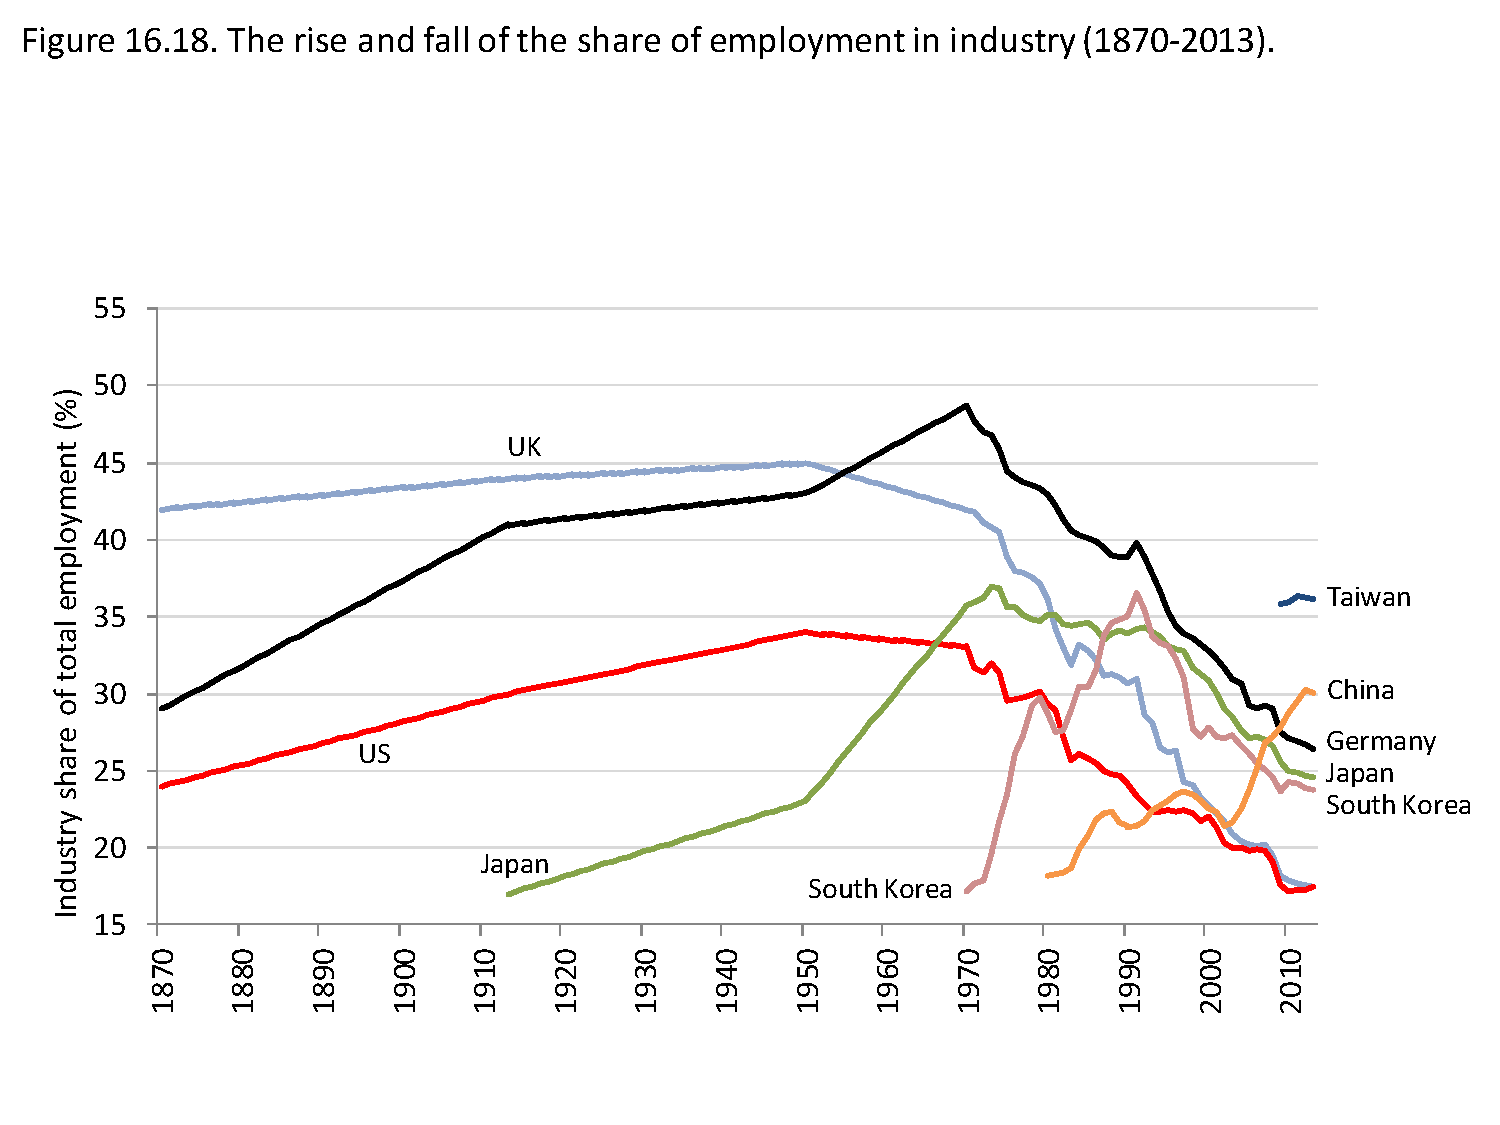
\includegraphics[trim={0cm, 1.8cm, 0cm, 5cm}, clip, width=\textwidth]{./figures/17.pdf}
    \end{figure}

        Countries get richer, industry moves:

        agriculture $ \rightarrow  $ manufacturing $ \rightarrow  $ services.

\end{frame}

\begin{frame}{Modelling shifts in production}
\label{slide:Modelling_shifts_in_production}
    \begin{figure}
        \centering
        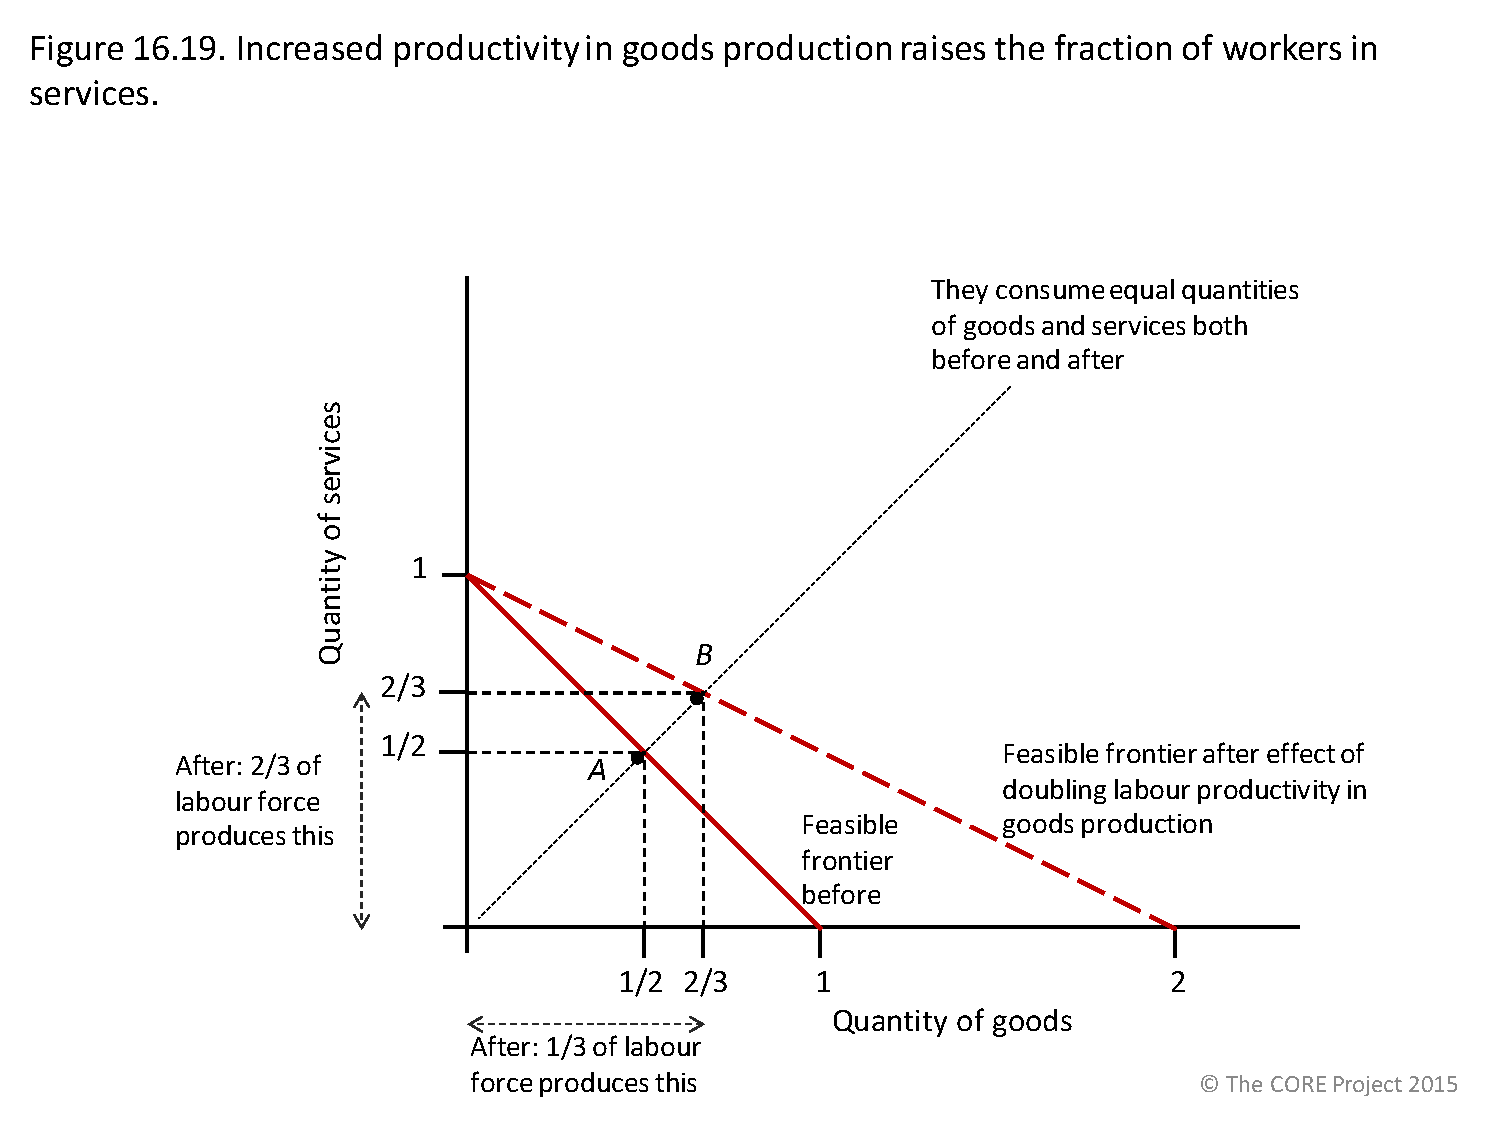
\includegraphics[trim = {0cm, 0cm, 0cm, 4.5cm}, clip, width=\textwidth]{./figures/18.pdf}
        \caption{Labor has been moving out of manufacturing (high productivity) into services (low productivity)}
    \end{figure}

\end{frame}

\begin{frame}{Does shifts in production actually happen?}
\label{slide:Does_shifts_in_production_actually_happen_}
    Yes, but some offsetting factors are excluded from this model:
    \begin{itemize}
        \item<1-4> Productivity increases in some services – productivity advances have been large in music sharing and digital information.
        \item<2-4> Substitution of goods for services – if the relative price of a good falls, consumers typically increase the proportion consumed.
        \item<3-4> Increase in relative demand for services – as incomes rise, people may choose to spend more of their budget on services.
        \item<4-4> Import and export patterns – international trade and opportunities for specialization affect which sectors grow/decline.
    \end{itemize}

\end{frame}


%\section{Appendix}
%\label{sec:Appendix}

%\appendix
%% -------------------------------------------
%\setbeamertemplate{headline}
%{
%\setbeamercolor{section in head/foot}{fg=black, bg=white}
%\vskip1em \tiny \insertsectionnavigationhorizontal{1\paperwidth}{\hspace{0.50\paperwidth}}{}
%}
%%------------------------------------------
%% \begin{frame}\frametitle{}
%% \begin{columns}
%% \label{Appendix}
%% \column{1\linewidth}
%% \centering
%% {\Large \alert{Appendix}}
%% \end{columns}
%% \end{frame}
%%------------------------------------------
%\begin{frame}[allowframebreaks]{References}
%\footnotesize
%\bibliographystyle{$BIB_STYLE}
%\bibliography{$BIBFILE}
%\end{frame}

\end{document}
